\documentclass[12pt]{article}

\usepackage{fancyhdr} % Required for custom headers
\usepackage{lastpage} % Required to determine the last page for the footer
\usepackage{extramarks} % Required for headers and footers
\usepackage[usenames,dvipsnames]{color} % Required for custom colors
\usepackage{graphicx} % Required to insert images
\usepackage{listings} % Required for insertion of code
\usepackage{courier} % Required for the courier font
\usepackage{lipsum} % Used for inserting dummy 'Lorem ipsum' text into the template
\usepackage{amsmath}
\usepackage{amssymb}
\usepackage{caption}
\usepackage[dvipsnames]{xcolor}

% Margins
\topmargin=-0.45in
\evensidemargin=0in
\oddsidemargin=0in
\textwidth=6.5in
\textheight=9.0in
\headsep=0.25in
\headheight=15.0pt


\linespread{1.1} % Line spacing

% Set up the header and footer
\pagestyle{fancy}
\lhead{\hmwkAuthorName} % Top left header
\chead{\hmwkClass: \hmwkTitle} % Top center head
\cfoot{} % Bottom center footer
\rfoot{Page\ \thepage\ of\ \protect\pageref{LastPage}} % Bottom right footer
\renewcommand\headrulewidth{0.4pt} % Size of the header rule
\renewcommand\footrulewidth{0.4pt} % Size of the footer rule

\setlength\parindent{0pt} % Removes all indentation from paragraphs

%----------------------------------------------------------------------------------------
%	DOCUMENT STRUCTURE COMMANDS
%	Skip this unless you know what you're doing
%----------------------------------------------------------------------------------------

% Header and footer for when a page split occurs within a problem environment
\newcommand{\enterProblemHeader}[1]{
	\nobreak\extramarks{#1}{#1 continued on next page\ldots}\nobreak
	\nobreak\extramarks{#1 (continued)}{#1 continued on next page\ldots}\nobreak
}

% Header and footer for when a page split occurs between problem environments
\newcommand{\exitProblemHeader}[1]{
	\nobreak\extramarks{#1 (continued)}{#1 continued on next page\ldots}\nobreak
	\nobreak\extramarks{#1}{}\nobreak
}

\setcounter{secnumdepth}{0} % Removes default section numbers
\newcounter{homeworkProblemCounter} % Creates a counter to keep track of the number of problems

\newcommand{\homeworkProblemName}{}
\newenvironment{homeworkProblem}[1][Problem \arabic{homeworkProblemCounter}]{ % Makes a new environment called homeworkProblem which takes 1 argument (custom name) but the default is "Problem #"
	\stepcounter{homeworkProblemCounter} % Increase counter for number of problems
	\renewcommand{\homeworkProblemName}{#1} % Assign \homeworkProblemName the name of the problem
	\section{\homeworkProblemName} % Make a section in the document with the custom problem count
	\enterProblemHeader{\homeworkProblemName} % Header and footer within the environment
}{
	\exitProblemHeader{\homeworkProblemName} % Header and footer after the environment
}

\newcommand{\problemAnswer}[1]{ % Defines the problem answer command with the content as the only argument
	\noindent\framebox[\columnwidth][c]{\begin{minipage}{0.98\columnwidth}#1\end{minipage}} % Makes the box around the problem answer and puts the content inside
}

\newcommand{\homeworkSectionName}{}
\newenvironment{homeworkSection}[1]{ % New environment for sections within homework problems, takes 1 argument - the name of the section
	\renewcommand{\homeworkSectionName}{#1} % Assign \homeworkSectionName to the name of the section from the environment argument
	\subsection{\homeworkSectionName} % Make a subsection with the custom name of the subsection
	\enterProblemHeader{\homeworkProblemName\ [\homeworkSectionName]} % Header and footer within the environment
}{
	\enterProblemHeader{\homeworkProblemName} % Header and footer after the environment
}

%----------------------------------------------------------------------------------------
%	NAME AND CLASS SECTION
%----------------------------------------------------------------------------------------

\newcommand{\hmwkTitle}{Assignment\ \#3} % Assignment title
\newcommand{\hmwkClass}{Advanced Image Processing} % Course/class
\newcommand{\hmwkClassInstructor}{Jones} % Teacher/lecturer
\newcommand{\hmwkAuthorName}{Shikhar Vashishth} % Your name
\newcommand{\hmwkAuthorID}{M.Tech CSA - 13374} % Your ID

%----------------------------------------------------------------------------------------
%	TITLE PAGE
%----------------------------------------------------------------------------------------

\title{
	\vspace{2in}
	\textmd{\textbf{\hmwkClass}}\\ 
	\textmd{\textbf{\hmwkTitle}}\\
	\vspace{3in}
}

\author{\textbf{\hmwkAuthorName} \\ {\small \hmwkAuthorID}}
\date{} % Insert date here if you want it to appear below your name

%----------------------------------------------------------------------------------------

\begin{document}
	
\maketitle
\newpage

\begin{homeworkProblem}
\subsection{Part (1):}

\begin{figure}[h]
	\centering
	\fbox{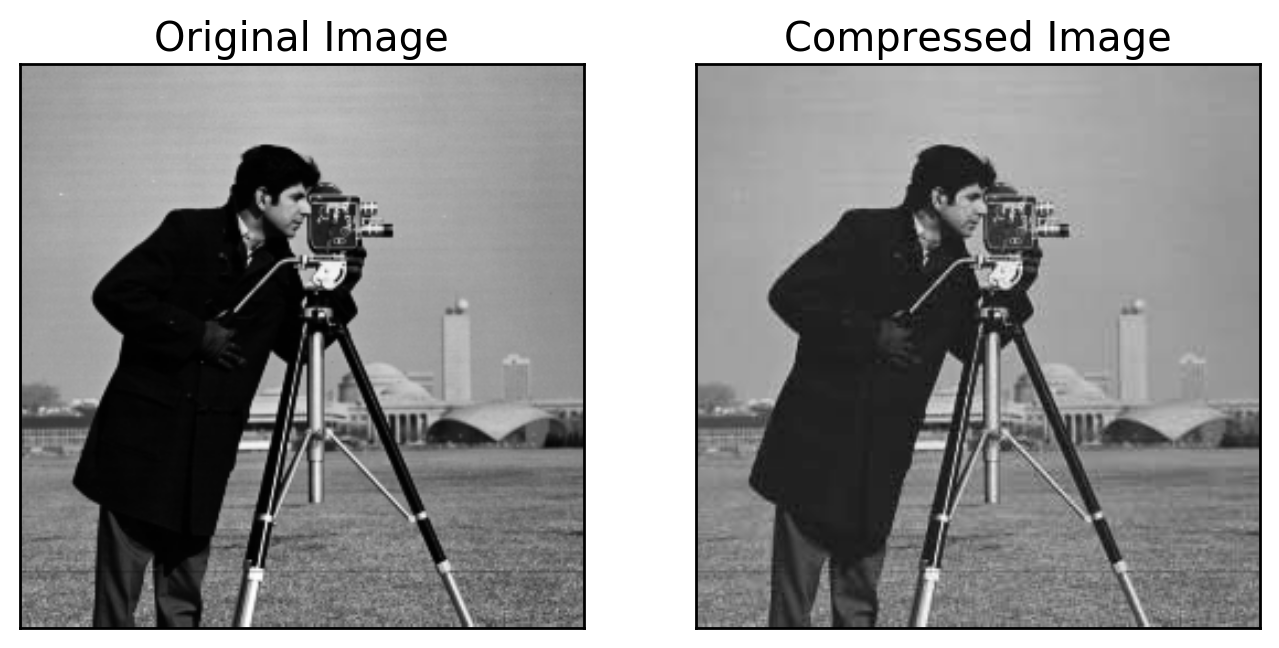
\includegraphics[width=12cm]{../Images/p1a.png}}
	\caption{Visual comparison of original and compressed Image}
\end{figure}

Size of the original Image: $521920$ bits \\
Size of the image after compression: $104486$ bits. \\
Mean square error: $38.70046$\\
Compression ratio = $\frac{\text{Size of input image}}{\text{Size of output image}} = \frac{521920}{104486} = 4.99511$

\subsubsection{Observations:}
\begin{enumerate}
	\item We can see from the above figure that although after compression the size of the image got reduced 5 times, but the visual appearance of the image did not deteriorate much. This shows the efficacy of JPEG algorithm in compression the image without corrupting its details.
	\item On closer analysis, one can find that the compressed image has some distortion near edges. This is because of the quantization matrix used during compression. Since the value of c chosen was large, therefore most of the high frequency component of the image got quantized to zero, which corrupted the edges little bit.
\end{enumerate}

\newpage
\subsection{Part (2):}

\begin{figure}[h]
	\centering
	\fbox{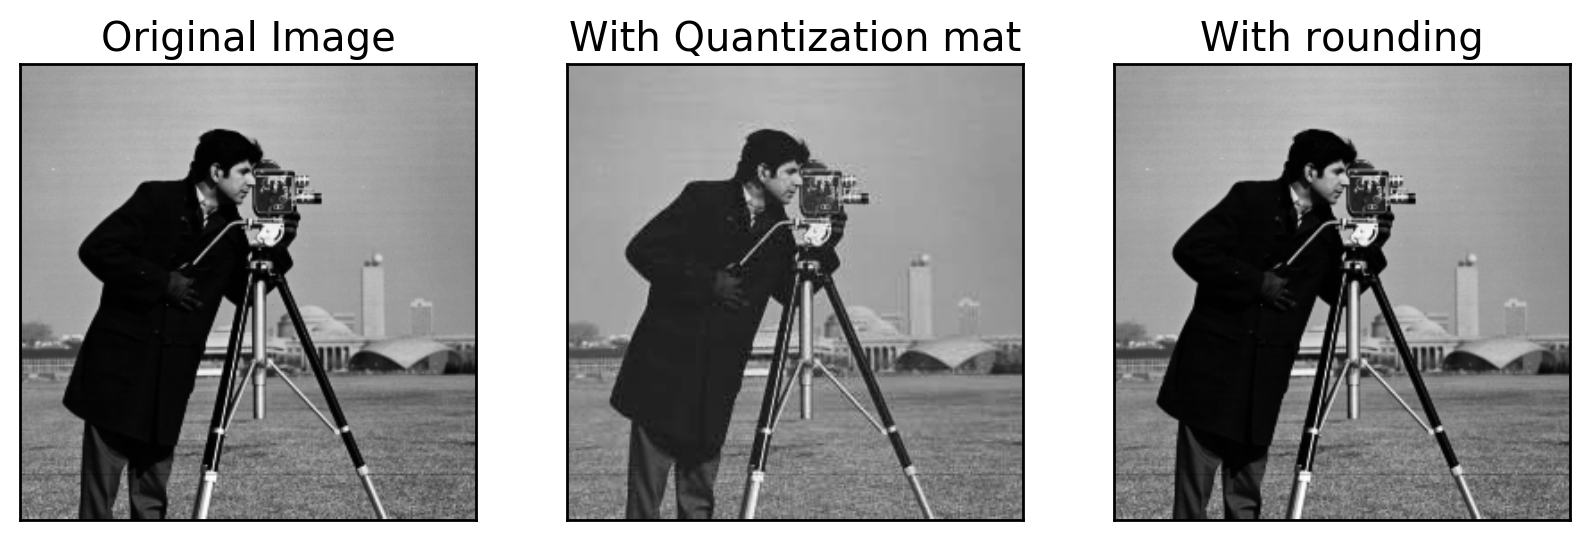
\includegraphics[width=16cm]{../Images/p1b.png}}
	\caption{Visual comparison of original and compressed Image}
\end{figure}

Size of the original Image: $521920$ bits \\
Size of the image after compression: $382052$ bits. \\
Mean square error: $0.08312$\\
Compression ratio = $\frac{\text{Size of input image}}{\text{Size of output image}} = \frac{521920}{382052} = 1.36608$


\subsubsection{Observations:}
\begin{enumerate}
	\item We can clearly see that without using the quantization matrix the compression ratio fell and the compressed image was found to be very close to the original image. This is because the high frequency component which doesn't considerably change the visual appearance of the output was not removed during the compression. So almost the entire image content was preserved which lead to poor compression.
\end{enumerate}

\newpage
\subsection{Part (3):}
\begin{figure}[h]
	\centering
	\fbox{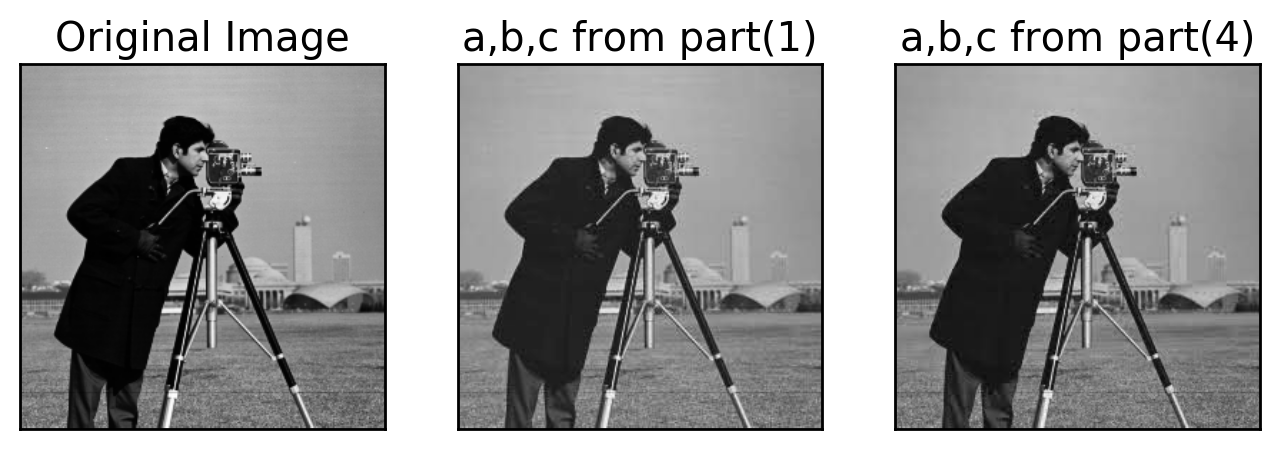
\includegraphics[width=\textwidth]{../Images/p1c.png}}
	\caption{Visual comparison of original and compressed Image}
\end{figure}

Best values of a, b, and c: 40, 30, and 30. \\
Size of the original Image: $521920$ bits \\
Size of the image after compression: $103786$ bits. \\
Mean square error: $32.52712$ (MSE part(1): 38.70046)\\
Compression ratio = $\frac{\text{Size of input image}}{\text{Size of output image}} = \frac{521920}{145988} = 5.0288092$

\subsubsection{Observations:}
\begin{enumerate}
	\item If we choose the values of a, b, and c as the smallest in the given range then we will get best possible MSE, but the compression ratio will be poor. This is because the smaller the values in the quantization matrix, more accurate is the reconstructed image. If the quantization matrix is chosen as all ones (like in the previous problem) the compression was poor and the image obtained after compression was almost identical to the original image. On the other hand, if we choose the values of a, b, and c to be the largest then, although we will get the maximum compression but the quality of obtained image is much worse. Therefore, the chosen value of a, b, and c lies somewhere in between.
	\item As we can see from the results, the MSE in this case is better than what we obtained in the part(1). This is because, although we increased the value of a from 20 to 40 but we have reduced the value of $b$ and $c$ which has allowed us to retain higher frequency component in the compressed image. Thus, giving us compressed image which is more closer to the original image visually and with lower MSE. In the part (1) we were using large value of c which was leading to distortion near the edges (high frequency component) of the image. But in the present case, we are using a smaller value of c, therefore no such distortion is experienced.
\end{enumerate}

\newpage
\subsection{Part (4):}
We know that for any distribution, Huffman codes gives the optimal length codeword in the case of lossless coding. So, if we can find a distribution for which the codes given in the table is the output of Huffman coding algorithm then we can say that codes given in the table for that distribution is the optimal. It turns out that there indeed exist such a distribution: \\ 

P(X = 0) = 1/2 \\
P(X = 1) = P(X = -1) = 1/8 \\
P(X = -3) = P(X = -2) = P(X = 2) = P(X = 3) = 1/32 \\
$....$ \\

Here $P(X=a)$ denotes the probability of occurrence of the number, $a$ in the distribution.
In general for any number $m$ the probability of occurrence can be defined as:
$$P(X=m) = \frac{1}{2^{\text{length of code}}}$$

Running Huffman coding algorithm on this distribution gives us the coding defined in the table. 

\paragraph{Example:} (here k represents rest of the numbers)
\begin{figure}[h]
	\centering
	\fbox{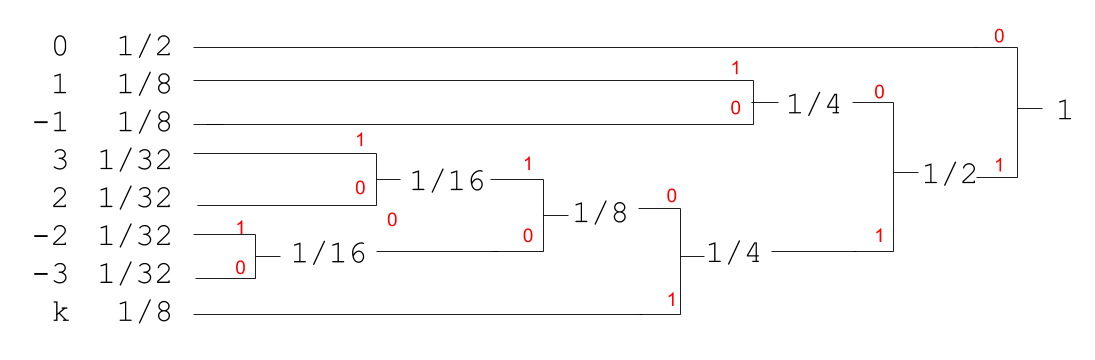
\includegraphics[width=\textwidth]{../Images/p1d.png}}
	\caption{Source distribution with optimal coding given in the table}
\end{figure}

\end{homeworkProblem}

\newpage
\begin{homeworkProblem}
We know that the mean of a uniformly distributed random variable is given by:
$$ \text{Mean} = \frac{a+b}{2}$$
Since, we know that the mean of both is zero, therefore:
$$\frac{a+b}{2} = 0 \implies a = -b$$

Variance of a uniformly distributed random variable is given by:
$$ \text{Variance} = \frac{(b-a)^2}{12}$$

We know that the variance of $X_1$ is $5$. Therefore:
$$ \frac{(b-a)^2}{12} = 5 \implies \frac{4a^2}{12} = 5 \implies a = \pm \sqrt{15}$$

So, $X_1$ is a uniform distribution from $-\sqrt{15}$ to $\sqrt{15}$. Similarly, we can show that $X_2$ is uniformly distribution from $-\sqrt{30}$ to $\sqrt{30}$. \\

The given budget constraint is:
$$ R_1 + R_2  = 3 \implies \log{K_1} + \log{K_2} = 3 \implies \log{K_1*K_2} = 3 \implies K_1*K_2 = 8$$

We know that the quantization points have to be positive integers, as having negative or fractional quantization points doesn't make sense. So, because of this constraint and the budget constraint there are only few possible values of $K_1$ and $K_2$ possible i.e. $(K_1, K_2) \in \{(1,8), (8,1), (4,2), (2,4	)\}$. Among these options we can check analytically which combination gives us the minimum error.

\subsubsection{Calculating expected error with $(K_1, K_2) = (2,4)$ :}

\begin{eqnarray*}
\mathbb{E}[(X_1 - \hat{X_1})^2] &=& \int_{-\sqrt{15}}^{\sqrt{15}} (x - \hat{x})^2f(x)dx \\
&=& \int_{-\sqrt{15}}^{0} (x + \sqrt{15}/2)^2\frac{1}{2\sqrt{15}}dx + \int_{0}^{\sqrt{15}} (x - \sqrt{15}/2)^2\frac{1}{2\sqrt{15}}dx \\
&=& \frac{5}{4}
\end{eqnarray*}

\begin{eqnarray*}
	\mathbb{E}[(X_2 - \hat{X_2})^2] &=& \int_{-\sqrt{30}}^{\sqrt{30}} (x - \hat{x})^2f(x)dx \\
	&=& \frac{1}{2\sqrt{30}} \left( \int_{-\sqrt{30}}^{-\sqrt{30}/2} (x + 3\sqrt{30}/4)^2dx + \int_{-\sqrt{30}/2}^{0} (x + \sqrt{30}/4)^2dx  \right) \\
	&+&  \frac{1}{2\sqrt{30}} \left( \int_{0}^{\sqrt{30}/2} (x - \sqrt{30}/4)^2dx + \int_{\sqrt{30}/2}^{\sqrt{30}} (x + 3\sqrt{30}/4)^2dx \right) \\
	&=& \frac{5}{8}
\end{eqnarray*}

\textbf{Total error: }
$$ \mathbb{E}[(X_1 - \hat{X_1})^2] + \mathbb{E}[(X_2 - \hat{X_2})^2] = \frac{5}{4} + \frac{5}{8} = 1.875$$

\subsubsection{Calculating expected error with $(K_1, K_2) = (4,2)$ :}
\begin{eqnarray*}
	\mathbb{E}[(X_1 - \hat{X_1})^2] &=& \int_{-\sqrt{15}}^{\sqrt{15}} (x - \hat{x})^2f(x)dx \\
	&=& \frac{1}{2\sqrt{15}} \left( \int_{-\sqrt{15}}^{-\sqrt{15}/2} (x + 3\sqrt{15}/4)^2dx + \int_{-\sqrt{15}/2}^{0} (x + \sqrt{15}/4)^2dx  \right) \\
	&+&  \frac{1}{2\sqrt{15}} \left( \int_{0}^{\sqrt{15}/2} (x - \sqrt{15}/4)^2dx + \int_{\sqrt{15}/2}^{\sqrt{15}} (x + 3\sqrt{15}/4)^2dx \right) \\
	&=& \frac{5}{16}
\end{eqnarray*}

\begin{eqnarray*}
	\mathbb{E}[(X_2 - \hat{X_2})^2] &=& \int_{-\sqrt{30}}^{\sqrt{30}} (x - \hat{x})^2f(x)dx \\
	&=& \int_{-\sqrt{30}}^{0} (x + \sqrt{30}/2)^2\frac{1}{2\sqrt{30}}dx + \int_{0}^{\sqrt{30}} (x - \sqrt{30}/2)^2\frac{1}{2\sqrt{30}}dx \\
	&=& \frac{5}{2}
\end{eqnarray*}

\textbf{Total error: }
$$ \mathbb{E}[(X_1 - \hat{X_1})^2] + \mathbb{E}[(X_2 - \hat{X_2})^2] = \frac{5}{16} + \frac{5}{2} = 2.8125$$

\subsubsection{Calculating expected error with $(K_1, K_2) = (1,8)$ :}
\begin{eqnarray*}
	\mathbb{E}[(X_1 - \hat{X_1})^2] &=& \int_{-\sqrt{15}}^{\sqrt{15}} (x - \hat{x})^2f(x)dx \\
	&=& \int_{-\sqrt{15}}^{\sqrt{15}} x^2\frac{1}{2\sqrt{15}}dx \\
	&=& 5
\end{eqnarray*}

We can see that for this choice the $\mathbb{E}[(X_1 - \hat{X_1})^2]$ exceeds the error in case of 1st choice. Hence, we can conclude that this is not a good choice.

\subsubsection{Calculating expected error with $(K_1, K_2) = (8,1)$ :}
\begin{eqnarray*}
	\mathbb{E}[(X_2 - \hat{X_2})^2] &=& \int_{-\sqrt{30}}^{\sqrt{30}} (x - \hat{x})^2f(x)dx \\
	&=& \int_{-\sqrt{30}}^{\sqrt{30}} x^2\frac{1}{2\sqrt{30}}dx \\
	&=& 10
\end{eqnarray*}

We can see that for this choice the $\mathbb{E}[(X_2 - \hat{X_2})^2]$ exceeds the error in case of 1st choice. Hence, we can conclude here itself that this is not a good choice.

\subsubsection{Conclusion:}
Therefore, we can conclude that the best choice of $K_1$ and $K_2$ is 2 and 4 because it gives us the minimum possible error as shown above.

\subsubsection{Relation of $(R_1, R_2)$ wrt a,b,c}
In the previous problem, the trade-off was between accurately quantizing low frequency and high frequency components, whereas in the present case there is a trade-off between accurately quantizing $X_1$ and $X_2$. To get low error, here we assigned more number of quantization levels to $X_2$ because its variance was large, similarly, in the previous problem also we gave more quantization levels to high frequency components than low frequency component because the variance of high frequency component is higher than that of low frequency component.
\end{homeworkProblem}

\end{document}